\chapter[Definiciones ]{Definiciones }\label{ch:capitulo3}
En este capítulo se presentan diversos términos fundamentales que se utilizaran en capítulos posteriores.

\subsection{Histogram of Gradient}
\label{subsec:hog}
Histogram of Oriented Gradients (HOG) are feature descriptors used in computer vision and image processing for the purpose of object detection. The technique counts occurrences of gradient orientation in localized portions of an image. This method is similar to that of edge orientation histograms, scale-invariant feature transform descriptors, and shape contexts, but differs in that it is computed on a dense grid of uniformly spaced cells and uses overlapping local contrast normalization for improved accuracy.

Navneet Dalal and Bill Triggs, researchers for the French National Institute for Research in Computer Science and Control (INRIA), first described Histogram of Oriented Gradient descriptors in their June 2005 CVPR paper. In this work they focused their algorithm on the problem of pedestrian detection in static images, although since then they expanded their tests to include human detection in film and video, as well as to a variety of common animals and vehicles in static imagery.

\begin{figure}[h]
  \centering
   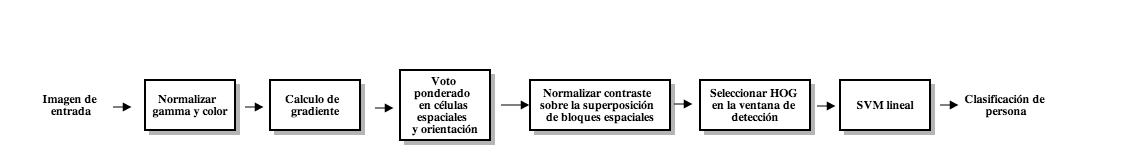
\includegraphics[width=1\textwidth]{Figuras/hog-procedure.png}
   \caption{Esquema de anotación}
   \label{fig:anota}
\end{figure}

\subsection{Filtros lineales}
\label{subsec:fl}

\subsection{Score}
\label{subsec:score}

\subsection{SVM}